% !TeX program = xelatex
\documentclass[a4paper,10pt]{article}

% ============================================================================
% កញ្ចប់បណ្ណាល័យ (Packages) – តាមលំនាំស្តង់ដារ អនុវិទ្យាល័យព្រះក្រសាំង (ls_plan.tex)
% បរិបទ៖ ថ្នាក់រៀនគ្មានស្លាយ LCD – បង្រៀនដោយប្រើក្ដារខៀន និងសន្លឹកកិច្ចការសិស្សស-ខ្មៅជាគោល
% ============================================================================
\usepackage[a4paper, left=0.95cm, right=0.95cm, top=0.85cm, bottom=0.92cm, footskip=0.52cm]{geometry}
\usepackage{amsmath}
\usepackage{unicode-math}
\usepackage{fontspec}
\usepackage{array, longtable, multirow, colortbl}
\usepackage[table]{xcolor}
\usepackage{enumitem}
\usepackage{pifont}
\usepackage{fancyhdr}
\usepackage{tikz}
\usetikzlibrary{calc, arrows.meta, angles, quotes, decorations.markings, positioning, babel}

\makeatletter
\let\@expl@@@mark@update@singlecol@structures@@\relax
\makeatother

% ============================================================================
% ការកំណត់ពុម្ពអក្សរផ្លូវការ (Cross-Platform Fonts Configuration)
% ============================================================================
\providecommand{\NGSFindFonts}{%
  \IfFileExists{C:/Windows/Fonts/cambria.ttc}{%
    \def\NGSSysPath{C:/Windows/Fonts/}%
    \def\NGSUserPath{C:/Users/KIT/AppData/Local/Microsoft/Windows/Fonts/}%
  }{%
    \IfFileExists{./fonts/KhmerOSsiemreap.ttf}{\def\NGSSysPath{./fonts/}\def\NGSUserPath{./fonts/}}{%
    \IfFileExists{../fonts/KhmerOSsiemreap.ttf}{\def\NGSSysPath{../fonts/}\def\NGSUserPath{../fonts/}}{%
    \IfFileExists{../../fonts/KhmerOSsiemreap.ttf}{\def\NGSSysPath{../../fonts/}\def\NGSUserPath{../../fonts/}}{%
    \IfFileExists{../../../fonts/KhmerOSsiemreap.ttf}{\def\NGSSysPath{../../../fonts/}\def\NGSUserPath{../../../fonts/}}{%
    \IfFileExists{../../../../fonts/KhmerOSsiemreap.ttf}{\def\NGSSysPath{../../../../fonts/}\def\NGSUserPath{../../../../fonts/}}{%
    \IfFileExists{../../../../../fonts/KhmerOSsiemreap.ttf}{\def\NGSSysPath{../../../../../fonts/}\def\NGSUserPath{../../../../../fonts/}}{%
    \IfFileExists{../../../../../../fonts/KhmerOSsiemreap.ttf}{\def\NGSSysPath{../../../../../../fonts/}\def\NGSUserPath{../../../../../../fonts/}}{%
      \def\NGSSysPath{../../../../../../../fonts/}\def\NGSUserPath{../../../../../../../fonts/}%
    }}}}}}}%
  }%
}
\NGSFindFonts

\setmathfont[Path={\NGSSysPath}, FontIndex=1, Scale=1.02]{cambria.ttc}
\defaultfontfeatures{Ligatures=TeX}

\setmainfont[
  Path={\NGSUserPath},
  Extension=.ttf,
  Script=Khmer,
  BoldFont={KhmerOSsiemreap},
  BoldFeatures={FakeBold=1.8},
  ItalicFont={KhmerOSsiemreap},
  ItalicFeatures={FakeSlant=0.25},
  BoldItalicFont={KhmerOSsiemreap},
  BoldItalicFeatures={FakeBold=1.8, FakeSlant=0.25}
]{KhmerOSsiemreap}

\newfontfamily\muol[Path={\NGSUserPath}, Extension=.ttf, Script=Khmer]{KhmerOSmuollight}
\newfontfamily\TimesEn[Path={\NGSSysPath}, Extension=.ttf, BoldFont={timesbd}, ItalicFont={timesi}, BoldItalicFont={timesbi}]{times}
\newfontfamily\NagaBold[Path={\NGSUserPath}, Extension=.ttf]{AKbalthom Naga Bold}
\newfontfamily\CalibriFont[Path={\NGSSysPath}, Extension=.ttf]{calibri}
\newfontfamily\Tacteing[Path={\NGSUserPath}]{TACTENG.TTF}
\newfontfamily\CourierBullet[Path={\NGSSysPath}, Extension=.ttf]{cour}
\newcommand{\wcirc}{{\CourierBullet\fontsize{9.5pt}{11pt}\selectfont o}}

\XeTeXlinebreaklocale "km"
\XeTeXlinebreakskip = 0pt plus 1pt minus 0.1pt

\definecolor{stepgray}{HTML}{D9D9D9}
\definecolor{headgray}{HTML}{F2F2F2}
\definecolor{boxgray}{HTML}{D9D9D9}
\definecolor{darkred}{HTML}{C00000}
\definecolor{red5e}{HTML}{FF0000}

\pagestyle{fancy}
\fancyhf{}
\renewcommand{\headrulewidth}{0pt}
\fancyfoot[R]{\CalibriFont\fontsize{11pt}{13pt}\selectfont\thepage}

\setlength{\parindent}{0pt}
\setlength{\parskip}{0pt}
\setlength{\tabcolsep}{3.8pt}

\newcolumntype{L}[1]{>{\raggedright\arraybackslash}p{#1}}

\newcommand{\en}[1]{{\TimesEn #1}}
\newcommand{\enbf}[1]{{\TimesEn\textbf{#1}}}
\newcommand{\unit}[1]{\,\text{\en{#1}}}
\newcommand{\fiveE}[1]{{\NagaBold\fontsize{9.5pt}{13pt}\selectfont\textcolor{red5e}{#1}}}
\newcommand{\timenote}[1]{\textcolor{darkred}{\textit{#1}}}
\newcommand{\redsub}[1]{\textcolor{darkred}{#1}}
\newcommand{\graybox}[1]{\colorbox{boxgray}{\strut\hspace{2pt}#1\hspace{2pt}}}
\newcommand{\ditem}{\tikz[baseline=-0.5ex]\fill (0,0.42ex) -- (0.42ex,0) -- (0,-0.42ex) -- (-0.42ex,0) -- cycle;\hspace{0.3em}}
\newcommand{\cnum}[1]{{\fontsize{10.5pt}{12pt}\selectfont\ding{\numexpr171+#1\relax}}\hspace{0.2em}}
\newcommand{\cfig}[1]{\par\vspace{4pt}{\centering #1\par}\vspace{4pt}}
\newcommand{\stepheader}[1]{\multicolumn{3}{|c|}{\cellcolor{stepgray}\muol #1} \\* \noalign{\hrule height 0.4pt}}
\newcommand{\tri}[1]{\ensuremath{\triangle #1}}
\newcommand{\ang}[1]{\ensuremath{\angle #1}}
\newcommand{\cg}{\ensuremath{\cong}}
\newcommand{\khmflourish}{{\Tacteing\fontsize{36pt}{14pt}\selectfont\raisebox{-5pt}{3}}}

\tikzset{
  tk1/.style={postaction={decorate},decoration={markings,mark=at position 0.50 with {\draw[black, line width=0.85pt](0,-0.095)--(0,0.095);}}},
  tk2/.style={postaction={decorate},decoration={markings,
    mark=at position 0.45 with {\draw[black, line width=0.85pt](0,-0.095)--(0,0.095);},
    mark=at position 0.55 with {\draw[black, line width=0.85pt](0,-0.095)--(0,0.095);}}},
  tk3/.style={postaction={decorate},decoration={markings,
    mark=at position 0.42 with {\draw[black, line width=0.85pt](0,-0.095)--(0,0.095);},
    mark=at position 0.50 with {\draw[black, line width=0.85pt](0,-0.095)--(0,0.095);},
    mark=at position 0.58 with {\draw[black, line width=0.85pt](0,-0.095)--(0,0.095);}}},
  par1/.style={postaction={decorate},decoration={markings,mark=at position 0.52 with {\draw[black, line width=0.85pt](-0.07,0.08)--(0.05,0)--(-0.07,-0.08);}}},
  par2/.style={postaction={decorate},decoration={markings,
    mark=at position 0.46 with {\draw[black, line width=0.85pt](-0.07,0.08)--(0.05,0)--(-0.07,-0.08);},
    mark=at position 0.58 with {\draw[black, line width=0.85pt](-0.07,0.08)--(0.05,0)--(-0.07,-0.08);}}}
}

% ============================================================================
% ម៉ាក្រូរូបភាពធរណីមាត្រស-ខ្មៅ (Proportional 4.0–7.2 cm B&W TikZ Diagrams)
% ============================================================================

% ១. រំលឹកមេរៀនទាក់ទង៖ លក្ខណៈបន្ទាត់ស្របច្រាស + លក្ខណៈត្រីកោណប៉ុនគ្នា ជ-ជ-ជ និង ជ-ម-ជ
\newcommand{\figPrereqPARATWO}{%
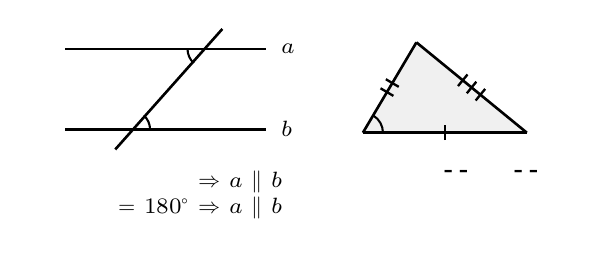
\begin{tikzpicture}[scale=0.85, every node/.style={font=\footnotesize, text=black}]
  % ឆ្វេង៖ មុំឆ្លាស់ក្នុងស្មើគ្នា => បន្ទាត់ស្រប
  \begin{scope}[shift={(0,0)}]
    \draw[black, line width=0.95pt] (0,1.35) -- (3.0,1.35) node[right=2pt] {$a$};
    \draw[black, line width=0.95pt] (0,0.15) -- (3.0,0.15) node[right=2pt] {$b$};
    \draw[black, line width=0.95pt] (2.35,1.65) -- (0.75,-0.15);
    \draw[black, line width=0.75pt] ($(2.11,1.35)+(180:0.28)$) arc (180:228:0.28);
    \draw[black, line width=0.75pt] ($(0.99,0.15)+(0:0.28)$) arc (0:48:0.28);
    \node[anchor=north, text width=3.35cm, align=center] at (1.55,-0.32) {មុំឆ្លាស់ក្នុងស្មើគ្នា $\Rightarrow a \parallel b$\\មុំរួមខាង $=180^\circ \Rightarrow a \parallel b$};
  \end{scope}
  % ស្ដាំ៖ លក្ខណៈ ជ-ជ-ជ និង ជ-ម-ជ
  \begin{scope}[shift={(4.45,0.10)}]
    \coordinate (P) at (0,0); \coordinate (Q) at (2.45,0); \coordinate (R) at (0.80,1.35);
    \fill[gray!12] (P)--(Q)--(R)--cycle;
    \draw[black, line width=0.95pt, tk1] (P)--(Q);
    \draw[black, line width=0.95pt, tk2] (P)--(R);
    \draw[black, line width=0.95pt, tk3] (R)--(Q);
    \draw[black, line width=0.75pt] ($(P)+(0:0.30)$) arc (0:59:0.30);
    \node[anchor=north, text width=3.35cm, align=center] at (1.22,-0.42) {លក្ខណៈប៉ុនគ្នា \textbf{ជ-ជ-ជ} និង \textbf{ជ-ម-ជ}};
  \end{scope}
\end{tikzpicture}}

% ២. E1 Engage: អន្ទាក់គូជ្រុងចម្រុះ (ប្រលេឡូក្រាម ទល់នឹង ចតុកោណព្នាយសមបាត)
\newcommand{\figEngagePARATWO}{%
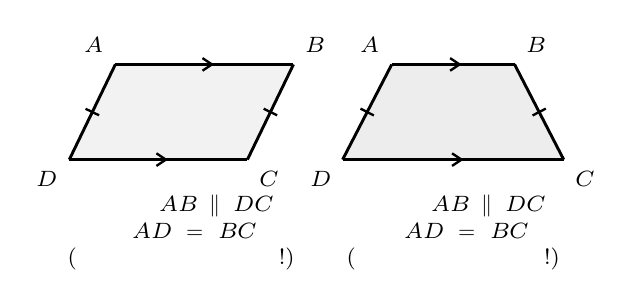
\begin{tikzpicture}[scale=0.78, every node/.style={font=\footnotesize, text=black}]
  % ឆ្វេង៖ ការរំពឹងទុករបស់កូនជាង (ប្រលេឡូក្រាម)
  \begin{scope}[shift={(0,0)}]
    \coordinate (D) at (0,0); \coordinate (C) at (2.90,0);
    \coordinate (A) at (0.75,1.55); \coordinate (B) at (3.65,1.55);
    \fill[gray!10] (A)--(B)--(C)--(D)--cycle;
    \draw[black, line width=1.05pt, par1] (A)--(B);
    \draw[black, line width=1.05pt, par1] (D)--(C);
    \draw[black, line width=1.05pt, tk1] (D)--(A);
    \draw[black, line width=1.05pt, tk1] (C)--(B);
    \node[above left=1pt] at (A) {$A$}; \node[above right=1pt] at (B) {$B$};
    \node[below right=1pt] at (C) {$C$}; \node[below left=1pt] at (D) {$D$};
    \node[anchor=north, text width=3.45cm, align=center] at (1.82,-0.42) {ទម្រង់ទី១៖ $AB\parallel DC$ និង $AD=BC$\\(កូនជាង ក ថា៖ ប្រលេឡូក្រាមដាច់ខាត!)};
  \end{scope}
  % ស្ដាំ៖ ឧទាហរណ៍ផ្ទុយរបស់មេជាង (ចតុកោណព្នាយសមបាត!)
  \begin{scope}[shift={(4.45,0)}]
    \coordinate (D) at (0,0); \coordinate (C) at (3.60,0);
    \coordinate (A) at (0.80,1.55); \coordinate (B) at (2.80,1.55);
    \fill[gray!14] (A)--(B)--(C)--(D)--cycle;
    \draw[black, line width=1.05pt, par1] (A)--(B);
    \draw[black, line width=1.05pt, par1] (D)--(C);
    \draw[black, line width=1.05pt, tk1] (D)--(A);
    \draw[black, line width=1.05pt, tk1] (C)--(B);
    \node[above left=1pt] at (A) {$A$}; \node[above right=1pt] at (B) {$B$};
    \node[below right=1pt] at (C) {$C$}; \node[below left=1pt] at (D) {$D$};
    \node[anchor=north, text width=3.45cm, align=center] at (1.80,-0.42) {ទម្រង់ទី២៖ $AB\parallel DC$ និង $AD=BC$\\(មេជាង ខ៖ អាចក្លាយជាចតុកោណព្នាយ!)};
  \end{scope}
\end{tikzpicture}}

% ៣. E3 Explain: សង្ខេបទ្រឹស្ដីបទសម្គាល់ប្រលេឡូក្រាម ទី៤–៧ (ទំ.១៧១–១៧៣)
\newcommand{\figTheoremsPARATWO}{%
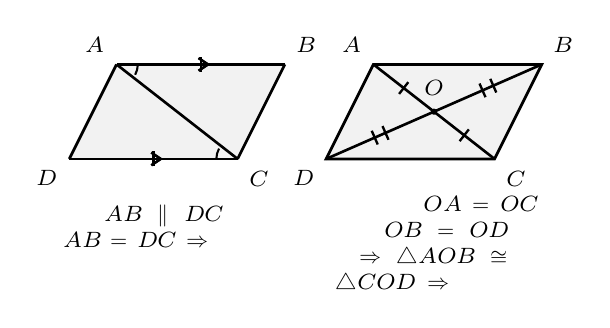
\begin{tikzpicture}[scale=0.75, every node/.style={font=\footnotesize, text=black}]
  % ឆ្វេង៖ ទ្រឹស្ដីបទទី៤ & ទី៦ (តាមអង្កត់ទ្រូង AC)
  \begin{scope}[shift={(0,0)}]
    \coordinate (D) at (0,0); \coordinate (C) at (2.85,0);
    \coordinate (A) at (0.80,1.60); \coordinate (B) at (3.65,1.60);
    \fill[gray!10] (A)--(B)--(C)--(D)--cycle;
    \draw[black, line width=1.0pt, par1, tk1] (A)--(B);
    \draw[black, line width=1.0pt, par1, tk1] (D)--(C);
    \draw[black, line width=1.0pt] (D)--(A) (C)--(B);
    \draw[black, line width=0.95pt] (A)--(C);
    \draw[black, line width=0.75pt] ($(A)+(-29:0.36)$) arc (-29:0:0.36);
    \draw[black, line width=0.75pt] ($(C)+(151:0.36)$) arc (151:180:0.36);
    \node[above left=1pt] at (A) {$A$}; \node[above right=1pt] at (B) {$B$};
    \node[below right=1pt] at (C) {$C$}; \node[below left=1pt] at (D) {$D$};
    \node[anchor=north, text width=3.45cm, align=center] at (1.82,-0.45) {ទ្រឹស្ដីបទទី៦៖ គូជ្រុងឈម\textbf{តែមួយ}\\$AB\parallel DC$ និង $AB=DC \Rightarrow$ ប្រលេឡូក្រាម};
  \end{scope}
  % ស្ដាំ៖ ទ្រឹស្ដីបទទី៧ (អង្កត់ទ្រូងកាត់គ្នាត្រង់ចំណុចកណ្ដាលនីមួយៗ O)
  \begin{scope}[shift={(4.35,0)}]
    \coordinate (D) at (0,0); \coordinate (C) at (2.85,0);
    \coordinate (A) at (0.80,1.60); \coordinate (B) at (3.65,1.60);
    \coordinate (O) at ($(A)!0.5!(C)$);
    \fill[gray!10] (A)--(B)--(C)--(D)--cycle;
    \draw[black, line width=1.0pt] (A)--(B)--(C)--(D)--cycle;
    \draw[black, line width=0.95pt, tk1] (A)--(O);
    \draw[black, line width=0.95pt, tk1] (O)--(C);
    \draw[black, line width=0.95pt, tk2] (B)--(O);
    \draw[black, line width=0.95pt, tk2] (O)--(D);
    \fill[black] (O) circle (1.5pt) node[above=2pt] {$O$};
    \node[above left=1pt] at (A) {$A$}; \node[above right=1pt] at (B) {$B$};
    \node[below right=1pt] at (C) {$C$}; \node[below left=1pt] at (D) {$D$};
    \node[anchor=north, text width=3.45cm, align=center] at (1.82,-0.45) {ទ្រឹស្ដីបទទី៧៖ $OA=OC$ និង $OB=OD$\\$\Rightarrow \tri{AOB}\cg\tri{COD} \Rightarrow$ ប្រលេឡូក្រាម};
  \end{scope}
\end{tikzpicture}}

% ៤. E4 Elaborate: លំហាត់គំរូទី១ (ទំ.១៧៣–១៧៤ ABEF & EFDC) និង គំរូទី២ (លំហាត់ទី៣ក ទំ.១៨៥)
\newcommand{\figModelPARATWO}{%
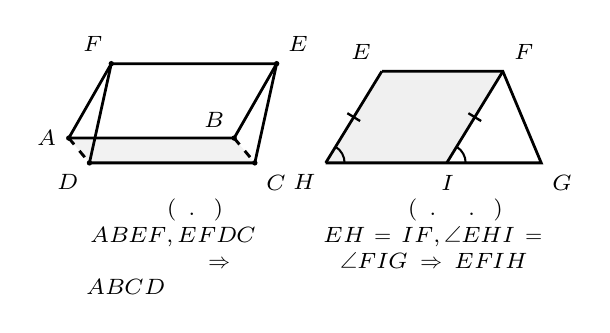
\begin{tikzpicture}[scale=0.75, every node/.style={font=\footnotesize, text=black}]
  % ឆ្វេង៖ លំហាត់គំរូសៀវភៅគោល ទំ.១៧៤ (ABEF និង EFDC ជាប្រលេឡូក្រាម)
  \begin{scope}[shift={(0,0)}]
    \coordinate (D) at (0.35,0);
    \coordinate (C) at (3.15,0);
    \coordinate (A) at (0,0.42);
    \coordinate (B) at (2.80,0.42);
    \coordinate (F) at (0.72,1.68);
    \coordinate (E) at (3.52,1.68);
    \fill[gray!10] (A)--(B)--(C)--(D)--cycle;
    \draw[black, line width=1.0pt] (F)--(E)--(B)--(A)--cycle;
    \draw[black, line width=1.0pt] (F)--(D)--(C)--(E);
    \draw[black, line width=1.05pt, dashed] (A)--(D) (B)--(C);
    \fill[black] (A) circle (1.3pt) node[left=1pt] {$A$};
    \fill[black] (B) circle (1.3pt) node[above left=0.5pt] {$B$};
    \fill[black] (C) circle (1.3pt) node[below right=1pt] {$C$};
    \fill[black] (D) circle (1.3pt) node[below left=1pt] {$D$};
    \fill[black] (F) circle (1.3pt) node[above left=1pt] {$F$};
    \fill[black] (E) circle (1.3pt) node[above right=1pt] {$E$};
    \node[anchor=north, text width=3.45cm, align=center] at (1.76,-0.45) {គំរូទី១ (ទំ.១៧៤)៖ $ABEF, EFDC$\\ជាប្រលេឡូក្រាម $\Rightarrow ABCD$ ជាប្រលេឡូក្រាម};
  \end{scope}
  % ស្ដាំ៖ លំហាត់ទី៣ក ទំ.១៨៥ (ចតុកោណ EFGH, I លើ HG)
  \begin{scope}[shift={(4.35,0)}]
    \coordinate (H) at (0,0);
    \coordinate (I) at (2.05,0);
    \coordinate (G) at (3.65,0);
    \coordinate (E) at (0.95,1.55);
    \coordinate (F) at (3.00,1.55);
    \fill[gray!12] (E)--(F)--(I)--(H)--cycle;
    \draw[black, line width=1.0pt, tk1] (H)--(E);
    \draw[black, line width=1.0pt, tk1] (I)--(F);
    \draw[black, line width=1.0pt] (E)--(F)--(G)--(H);
    \draw[black, line width=0.75pt] ($(H)+(0:0.32)$) arc (0:58:0.32);
    \draw[black, line width=0.75pt] ($(I)+(0:0.32)$) arc (0:58:0.32);
    \node[below left=1pt] at (H) {$H$};
    \node[below=1pt] at (I) {$I$};
    \node[below right=1pt] at (G) {$G$};
    \node[above left=1pt] at (E) {$E$};
    \node[above right=1pt] at (F) {$F$};
    \node[anchor=north, text width=3.45cm, align=center] at (1.82,-0.45) {គំរូទី២ (លំ.៣ក ទំ.១៨៥)៖\\$EH=IF, \ang{EHI}=\ang{FIG} \Rightarrow EFIH$};
  \end{scope}
\end{tikzpicture}}

% ៥. E5 Evaluate: ប្រតិបត្តិ ទំ.១៧៤ (ត្រីកោណ ABC, O កណ្ដាល BC, D ឆ្លុះ A ធៀប O)
\newcommand{\figPractPARATWO}{%
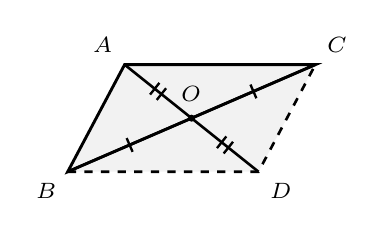
\begin{tikzpicture}[scale=0.85, every node/.style={font=\footnotesize, text=black}]
  \coordinate (B) at (0,0);
  \coordinate (D) at (2.85,0);
  \coordinate (A) at (0.85,1.60);
  \coordinate (C) at (3.70,1.60);
  \coordinate (O) at ($(B)!0.5!(C)$);
  \fill[gray!10] (A)--(B)--(D)--(C)--cycle;
  \draw[black, line width=1.05pt] (A)--(B)--(C)--cycle;
  \draw[black, line width=0.95pt, dashed] (B)--(D)--(C);
  \draw[black, line width=0.95pt, tk1] (B)--(O);
  \draw[black, line width=0.95pt, tk1] (O)--(C);
  \draw[black, line width=0.95pt, tk2] (A)--(O);
  \draw[black, line width=0.95pt, tk2] (O)--(D);
  \fill[black] (O) circle (1.5pt) node[above=2.5pt] {$O$};
  \node[above left=1pt] at (A) {$A$};
  \node[below left=1pt] at (B) {$B$};
  \node[above right=1pt] at (C) {$C$};
  \node[below right=1pt] at (D) {$D$};
\end{tikzpicture}}

\begin{document}
\fontsize{10pt}{15.2pt}\selectfont

% -------------------- ក្បាលកិច្ចតែងការ (Header) --------------------
\begin{center}
  {\muol\fontsize{11pt}{16pt}\selectfont ព្រះរាជាណាចក្រកម្ពុជា}\\[2pt]
  {\muol\fontsize{10pt}{15pt}\selectfont ជាតិ សាសនា ព្រះមហាក្សត្រ}\\[1pt]
  \khmflourish
\end{center}

\vspace{-28pt}
{\muol\fontsize{9.5pt}{12.5pt}\selectfont
មន្ទីរអប់រំ យុវជន និងកីឡា ខេត្តកំពង់ធំ\\
ការិយាល័យអប់រំ យុវជន និងកីឡា ស្រុកកំពង់ស្វាយ\\
អនុវិទ្យាល័យព្រះក្រសាំង}

\vspace{1pt}
\begin{center}
  {\muol\fontsize{10pt}{14pt}\selectfont កិច្ចតែងការបង្រៀន}
\end{center}
\vspace{0pt}

% -------------------- ព័ត៌មានទូទៅ (Metadata) --------------------
{\renewcommand{\arraystretch}{0.95}
\hspace*{4.05cm}%
\begin{tabular}{@{}l l l@{}}
  - \hspace{0.35cm} មុខវិជ្ជា & : & គណិតវិទ្យា ថ្នាក់ទី៨ \\
  - \hspace{0.35cm} ចំណងជើងមេរៀន & : & មេរៀនទី១៣ ចតុកោណ \\
  - \hspace{0.35cm} ចំណងជើងរង & : & ២.១.២ លក្ខណៈសម្គាល់ប្រលេឡូក្រាម៖ ទ្រឹស្ដីបទទី៤--៧ (ទំ.១៧១--១៧៤) \\
  - \hspace{0.35cm} រយៈពេល & : & ១ ម៉ោងសិក្សា (៥០ នាទី) \\
  - \hspace{0.35cm} បង្រៀនដោយ & : & ហុក ប៊ុនថែន \\
  - \hspace{0.35cm} កាលបរិច្ឆេទ & : & ថ្ងៃចន្ទ ៥កើត ខែមិគសិរ ព.ស.២៥៧០ (១៤ ធ្នូ ២០២៦) \\
\end{tabular}

\vspace{1pt}

% -------------------- I. វត្ថុបំណង --------------------
\textbf{I.} {\muol វត្ថុបំណង}\\[1pt]
\hspace*{0.55cm}%
\begin{tabular}{@{}l l L{14.2cm}@{}}
  \wcirc \hspace{0.25cm} វិជ្ជាសម្បទា & : & សិស្សពោលបានត្រឹមត្រូវនូវលក្ខណៈសម្គាល់ប្រលេឡូក្រាមទាំង ៥ ផ្លូវ គឺតាមនិយមន័យ ទ្រឹស្ដីបទទី៤ (ជ្រុងឈមប៉ុនគ្នាពីរៗ) ទ្រឹស្ដីបទទី៥ (មុំឈមប៉ុនគ្នាពីរៗ) ទ្រឹស្ដីបទទី៦ (គូជ្រុងឈមតែមួយស្របគ្នានិងប៉ុនគ្នា) និងទ្រឹស្ដីបទទី៧ (អង្កត់ទ្រូងកាត់គ្នាត្រង់ចំណុចកណ្ដាលរៀងគ្នា) តាមសៀវភៅគោល ទំ.១៧១--១៧៤ ។ \\
  \wcirc \hspace{0.25cm} បំណិនសម្បទា & : & សិស្សវិភាគបដិសេធលក្ខខណ្ឌមិនគ្រប់គ្រាន់ដោយឧទាហរណ៍ផ្ទុយ (ចតុកោណព្នាយសមបាត) បំពេញសម្រាយបញ្ជាក់ទ្រឹស្ដីបទទី៦--៧ លើសន្លឹកកិច្ចការស-ខ្មៅ និងស្រាយបញ្ជាក់ចតុកោណជាប្រលេឡូក្រាមក្នុងលំហាត់គំរូ និងប្រតិបត្តិដោយភ្ជាប់ធនាគារហេតុផល \cnum{1}--\cnum{5} ។ \\
  \wcirc \hspace{0.25cm} ចរិយាសម្បទា & : & សិស្សមានស្មារតីប្រុងប្រយ័ត្នផ្នែកតក្កវិទ្យា (មិនសន្និដ្ឋានប្រញាប់លើគូជ្រុងចម្រុះស្របមួយគូ-ស្មើមួយគូឡើយ) សហការពិភាក្សាជាដៃគូយ៉ាងសកម្ម និងផ្សារភ្ជាប់ទៅនឹងការផ្ទៀងផ្ទាត់ស៊ុមសំណង់ក្នុងជីវភាពពិត ។ \\
\end{tabular}

\vspace{1pt}

% -------------------- II. សម្ភារៈឧបទេស --------------------
\textbf{II.} {\muol សម្ភារៈឧបទេស}\\[1pt]
\hspace*{0.55cm}$\bullet$ \hspace{0.35cm} សៀវភៅសិក្សាគោលគណិតវិទ្យាថ្នាក់ទី៨ (ទំ.១៧១--១៧៤ និងទំ.១៨៥) ក្ដារខៀន ដីស បន្ទាត់ក្រិត ដែកឈាន និងសន្លឹកកិច្ចការសិស្សស-ខ្មៅ (\en{Worksheet\_PARA2} ចំនួន ២ ទំព័រ \en{A4} សម្រាប់វិភាគឧទាហរណ៍ផ្ទុយ និងបំពេញសម្រាយបញ្ជាក់ ដោយគ្មានស្លាយ \en{LCD}) ។

\vspace{1pt}

% -------------------- III. វិធីសាស្រ្តបង្រៀន --------------------
\textbf{III.} {\muol វិធីសាស្រ្តបង្រៀន}\\[1pt]
\hspace*{0.45cm}%
\begin{tabular}{@{}l l L{14.85cm}@{}}
  $\bullet$ \hspace{0.25cm} គោលវិធី & : & សិស្សមជ្ឈមណ្ឌល (សិក្សាស៊ើបអង្កេតជាដៃគូលើសន្លឹកកិច្ចការបំពេញផ្ទាល់ គ្មានស្លាយ \en{LCD}) \\
  $\bullet$ \hspace{0.25cm} យុទ្ធវិធីបង្រៀន & : & គម្រូស្ថាបនានិយម \en{5Es} រួមបញ្ចូល \textbf{ការបដិសេធដោយឧទាហរណ៍ផ្ទុយ និងការជម្រើសលក្ខខណ្ឌគ្រប់គ្រាន់អប្បបរមា} (\en{Counter-Example Refutation \& Minimal-Sufficiency Triage — Zaslavsky \& Shir, 2005}) \\
\end{tabular}
}

\vspace{1pt}

% -------------------- IV. ដំណើរការបង្រៀន --------------------
\textbf{IV.} {\muol ដំណើរការបង្រៀន}

\vspace{1pt}

\renewcommand{\arraystretch}{1.15}
\begin{longtable}{|L{5.50cm}|L{7.90cm}|L{4.80cm}|}
\hline
\rowcolor{headgray}
\multicolumn{1}{|c|}{\muol សកម្មភាពគ្រូ} &
\multicolumn{1}{c|}{\muol ខ្លឹមសារមេរៀន} &
\multicolumn{1}{c|}{\muol សកម្មភាពសិស្ស} \\
\hline
\endfirsthead
\hline
\endhead
\hline
\endfoot
\hline
\endlastfoot

% ==================== ជំហានទី១ (2min) ====================
\stepheader{ជំហានទី១ \enbf{(}រដ្ឋបាលថ្នាក់\enbf{)}}
$\bullet$ ពិនិត្យអវត្តមាន សណ្ដាប់ធ្នាប់ អនាម័យ និងការត្រៀមបន្ទាត់ក្រិត-ដែកឈាន
&
$\bullet$ ពិនិត្យវត្តមាន និងសណ្ដាប់ធ្នាប់ថ្នាក់រៀន \par
$\bullet$ ត្រៀមបន្ទាត់ក្រិត និងដែកឈានសម្រាប់សង្កេតលើសន្លឹកកិច្ចការ
&
$\circ$ ប្រធានថ្នាក់រាយការណ៍អវត្តមាន និងត្រៀមឧបករណ៍ធរណីមាត្រ \\[3pt]

$\bullet$ រៀបចំសិស្សជាដៃគូពិភាក្សា រួចចែកសន្លឹកកិច្ចការ \en{Worksheet\_PARA2} (២ ទំព័រ \en{A4}) ផ្កាប់លើតុ
&
$\bullet$ ការចាត់ដៃគូសិក្សា និងចែកសន្លឹកកិច្ចការស-ខ្មៅ
&
$\circ$ អង្គុយតាមដៃគូ និងទទួលសន្លឹកកិច្ចការទុកលើតុ \\
\hline

% ==================== ជំហានទី២ (9min: <=3 + 3 + E1 3) ====================
\stepheader{ជំហានទី២ \enbf{(}កិច្ចការផ្ទះ \enbf{+} ទំនាក់ទំនងមេរៀនថ្មី\enbf{)}}
\ditem \textbf{កំណែកិច្ចការផ្ទះ ($\le 3\unit{min}$)} \timenote{សង្ខេបខ្លីលើក្ដារខៀន}
&
{\centering\redsub{កំណែកិច្ចការផ្ទះ (លំហាត់ទី៥ និងទី៧ ទំ.១៨៥)}\par}
&
$\circ$ យកសៀវភៅកិច្ចការផ្ទះមកផ្ទៀងផ្ទាត់ \\[2pt]

$\bullet$ ផ្ទៀងផ្ទាត់ចម្លើយលំហាត់ទី៥ និងលទ្ធផល $OA'=OC', OB'=OD'$ នៃលំហាត់ទី៧
&
$\bullet$ \textbf{លំ.៥៖} $(2x+20^\circ)+(x-50^\circ)=180^\circ \Rightarrow 3x=210^\circ \Rightarrow x=70^\circ$ (មុំស្មើ $160^\circ$ និង $20^\circ$) ។ \par
$\bullet$ \textbf{លំ.៧៖} តាមទ្រឹស្ដីបទផ្ចិតឆ្លុះ គេបាន $OA'=OC'$ និង $OB'=OD'$ ។
&
$\circ$ ផ្ទៀងផ្ទាត់ចម្លើយ និងកត់ចំណាំទុកតភ្ជាប់ក្នុងមេរៀនថ្ងៃនេះ \\[3pt]

\ditem \textbf{រំលឹកមេរៀនទាក់ទង ($3\unit{min}$)} \par
$\bullet$ គូសរូបលើក្ដារខៀន សួររំលឹកទី១៖ តើយើងអាចបង្ហាញថាបន្ទាត់ពីរ $a$ និង $b$ ស្របគ្នាតាមរយៈមុំអ្វីខ្លះ?
&
{\centering\redsub{រំលឹកមេរៀនទាក់ទងមេរៀនថ្មី}\par} \par
$\bullet$ បើមុំឆ្លាស់ក្នុងស្មើគ្នា ឬមុំត្រូវគ្នាស្មើគ្នា ឬផលបូកមុំក្នុងរួមខាងស្មើ $180^\circ$ នោះបន្ទាត់ទាំងពីរ\textbf{ស្របគ្នា} ($a \parallel b$) ។
&
$\circ$ ឆ្លើយរំលឹកលក្ខណៈបន្ទាត់ស្របច្រាសតាមមុំឆ្លាស់ក្នុង និងមុំក្នុងរួមខាង \\[2pt]

– \textbf{សំណួរទី២៖} តើលក្ខណៈត្រីកោណប៉ុនគ្នា \textbf{ជ-ជ-ជ} និង \textbf{ជ-ម-ជ} ត្រូវការធាតុអ្វីខ្លះ?
&
$\bullet$ \textbf{ជ-ជ-ជ}៖ ជ្រុងទាំងបីស្មើគ្នារៀងគ្នា ។ \textbf{ជ-ម-ជ}៖ ជ្រុងពីរ និងមុំក្នុងចន្លោះជ្រុងទាំងពីរស្មើគ្នារៀងគ្នា ។
&
$\circ$ រំលឹកលក្ខណៈត្រីកោណប៉ុនគ្នា \textbf{ជ-ជ-ជ} និង \textbf{ជ-ម-ជ} \\[3pt]

&
\cfig{\figPrereqPARATWO}
& \\[3pt]

\fiveE{E1 - Engage (3min)} \timenote{(កុំទាន់ផ្ដល់ចម្លើយ)} \par
\ditem \textbf{បញ្ហាភ្ញាក់ផ្អើល «ស៊ុមទ្វារដែករបស់ជាងផ្សារដែក»៖} \par
$\bullet$ គូសរូបស៊ុមដែក $ABCD$ ដែលរបារលើ-ក្រោមស្របគ្នា ($AB\parallel DC$) ហើយរបារឆ្វេង-ស្ដាំស្មើគ្នា ($AD=BC=1.2\unit{m}$)
&
{\centering\redsub{ស្ថានភាពបញ្ហា៖ រោងជាងផ្សារដែកឃុំព្រះក្រសាំង}\par}
&
$\circ$ សង្កេតរូបប្រៀបធៀបទាំងពីរលើក្ដារខៀន និងលើក្បាលសន្លឹកកិច្ចការ \\[3pt]

&
\cfig{\figEngagePARATWO}
& \\[3pt]

– \textbf{សំណួរបំផុស៖} «កូនជាង ក អះអាងថា ឱ្យតែ $AB\parallel DC$ ហើយ $AD=BC$ ស៊ុមនេះច្បាស់ជាប្រលេឡូក្រាម ១០០\%! តែមេជាង ខ គ្រវីក្បាលថា អាចក្លាយជារាងព្នាយទៅវិញ! តើត្រូវកែលក្ខខណ្ឌយ៉ាងដូចម្ដេចទើបធានាបានប្រលេឡូក្រាមពិតប្រាកដ?»
&
\textbf{ចម្ងល់គោលប្រចាំម៉ោង៖} \par
តើលក្ខខណ្ឌអប្បបរមាណាខ្លះ (លើជ្រុង មុំ ឬអង្កត់ទ្រូង) ដែលគ្រប់គ្រាន់ធានាថាចតុកោណមួយជា\textbf{ប្រលេឡូក្រាម} ដោយគ្មានករណីលើកលែង?
&
$\circ$ ពិភាក្សាជាដៃគូ ៣០ វិនាទី រួចគូសធីកការទស្សន៍ទាយដំបូងក្នុងប្រអប់ \en{E1} លើសន្លឹកកិច្ចការ \\
\hline

% ==================== ជំហានទី៣ (17min: E2 11m + E3 6m) ====================
\stepheader{ជំហានទី៣ \enbf{(}ខ្លឹមសារមេរៀនថ្មី\enbf{)}}
\fiveE{E2 - Explore (11min)} \par
$\bullet$ សរសេរចំណងជើងរងលើក្ដារខៀន និងឱ្យសិស្សបើកសន្លឹកកិច្ចការទំព័រទី១ ផ្នែកទី២
&
២.១.២ លក្ខណៈសម្គាល់ប្រលេឡូក្រាម៖ ទ្រឹស្ដីបទទី៤--៧ (ទំ.១៧១--១៧៤)
&
$\circ$ កត់ចំណងជើងរងចូលសៀវភៅសរសេរ និងបើកសន្លឹកកិច្ចការទំព័រទី១ \\[3pt]

\ditem \textbf{សកម្មភាពទី១៖ តារាងជម្រើសលក្ខខណ្ឌ និងឧទាហរណ៍ផ្ទុយ ($5.5\unit{min}$)} \par
$\bullet$ ឱ្យដៃគូសិស្សពិនិត្យករណីសាកល្បងទាំង ៦ (ក--ច) លើសន្លឹកកិច្ចការ រួចសម្រេចថា «គ្រប់គ្រាន់» ឬ «មិនគ្រប់គ្រាន់ (មានឧទាហរណ៍ផ្ទុយ)»
&
{\centering\textbf{លទ្ធផលវិនិច្ឆ័យករណីសាកល្បងទាំង ៦}\par} \par
$\bullet$ \textbf{គ្រប់គ្រាន់ជាប្រលេឡូក្រាម (៤ ករណី)៖} \par
(ក) $AB=DC, AD=BC$ \quad (ខ) $\ang{A}=\ang{C}, \ang{B}=\ang{D}$ \par
(ឃ) $AB\parallel DC$ និង $AB=DC$ \quad (ង) $OA=OC$ និង $OB=OD$ ។
&
$\circ$ ពិនិត្យសញ្ញាឆ្នូត និងព្រួញស្របលើរូបទាំង ៦ ករណីជាដៃគូ \\[2pt]

$\bullet$ ហៅដៃគូសិស្សបង្ហាញករណីអន្ទាក់ (គ) និង (ច) ដែលមិនមែនជាប្រលេឡូក្រាម!
&
$\bullet$ \textbf{បំបែកការយល់ច្រឡំ (ឧទាហរណ៍ផ្ទុយ)៖} \par
– \textbf{ករណី គ ($AB\parallel DC$ តែ $AD=BC$)៖} \graybox{មិនគ្រប់គ្រាន់!} អាចជា\textbf{ចតុកោណព្នាយសមបាត} ។ \par
– \textbf{ករណី ច ($AC=BD$ ប៉ុណ្ណោះ)៖} \graybox{មិនគ្រប់គ្រាន់!} អង្កត់ទ្រូងស្មើគ្នាតែមិនចែកពាក់កណ្ដាលគ្នា ក៏អាចជាចតុកោណព្នាយសមបាតដែរ!
&
$\circ$ រកឃើញឧទាហរណ៍ផ្ទុយនៃចតុកោណព្នាយសមបាតក្នុងករណី (គ) និង (ច) \\[3pt]

\ditem \textbf{សកម្មភាពទី២៖ តារាងសម្រាយបញ្ជាក់ទ្រឹស្ដីបទទី៦ និងទី៧ ($5.5\unit{min}$)} \par
$\bullet$ ណែនាំឱ្យគូស \textbf{[tracing]} អង្កត់ទ្រូង $AC$ ដើម្បីបំពេញសម្រាយបញ្ជាក់ \textbf{ផ្នែក ក (ទ្រឹស្ដីបទទី៦)}៖ $AB\parallel DC$ និង $AB=DC$
&
\textbf{គោលគំនិតសម្រាយបញ្ជាក់ច្រាស៖} \par
$\bullet$ \textbf{ផ្នែក ក (ទ្រឹស្ដីបទទី៦)៖} គូស $AC$ ។ ក្នុង $\tri{ADC}$ និង $\tri{CBA}$ មាន៖ $DC=BA$, $\ang{ACD}=\ang{CAB}$ (ឆ្លាស់ក្នុងនៃ $AB\parallel DC$), $AC$ រួម $\Rightarrow \tri{ADC}\cg\tri{CBA}$ (\textbf{ជ-ម-ជ}) $\Rightarrow \ang{DAC}=\ang{BCA} \Rightarrow AD\parallel BC$ ។
&
$\circ$ គូស \textbf{[tracing]} អង្កត់ទ្រូង $AC$ និងបំពេញតារាងសម្រាយបញ្ជាក់ \textbf{ផ្នែក ក} \\[2pt]

$\bullet$ ណែនាំឱ្យផ្គូផ្គង $\tri{AOB}$ និង $\tri{COD}$ ដើម្បីបំពេញ \textbf{ផ្នែក ខ (ទ្រឹស្ដីបទទី៧)}៖ $OA=OC$ និង $OB=OD$
&
$\bullet$ \textbf{ផ្នែក ខ (ទ្រឹស្ដីបទទី៧)៖} $OA=OC$, $\ang{AOB}=\ang{COD}$ (ទល់កំពូល), $OB=OD \Rightarrow \tri{AOB}\cg\tri{COD}$ (\textbf{ជ-ម-ជ}) $\Rightarrow AB=CD$ និង $\ang{OAB}=\ang{OCD} \Rightarrow AB\parallel CD$ ។
&
$\circ$ បំពេញតារាងសម្រាយបញ្ជាក់ \textbf{ផ្នែក ខ} រហូតទាញបានប្រលេឡូក្រាម \\[3pt]

\fiveE{E3 - Explain (6min)} \par
\ditem \textbf{បង្គុំធនាគារហេតុផលសម្គាល់ប្រលេឡូក្រាម \cnum{1}--\cnum{5} (ទំ.១៧១--១៧៣)៖} \par
$\bullet$ ហៅតំណាងដៃគូឡើងបកស្រាយ រួចគ្រូសង្ខេបផ្លូវទាំង ៥ សម្រាប់បង្ហាញថាចតុកោណ $ABCD$ ជាប្រលេឡូក្រាម
&
\textbf{ធនាគារហេតុផលសម្គាល់ប្រលេឡូក្រាម \cnum{1}--\cnum{5}៖} \par
\cnum{1} \textbf{និយមន័យ៖} ជ្រុងឈមស្របគ្នាពីរៗ ($AB\parallel DC$ និង $AD\parallel BC$) ។ \par
\cnum{2} \textbf{ទ្រឹស្ដីបទទី៤៖} ជ្រុងឈមប៉ុនគ្នាពីរៗ ($AB=DC$ និង $AD=BC$, តាម \textbf{ជ-ជ-ជ}) ។ \par
\cnum{3} \textbf{ទ្រឹស្ដីបទទី៥៖} មុំឈមប៉ុនគ្នាពីរៗ ($\ang{A}=\ang{C}$ និង $\ang{B}=\ang{D} \Rightarrow 2\ang{A}+2\ang{B}=360^\circ \Rightarrow \ang{A}+\ang{B}=180^\circ$) ។
&
$\circ$ តំណាងដៃគូឡើងបកស្រាយ និងសិស្សបំពេញ \cnum{1}--\cnum{3} លើសន្លឹកកិច្ចការទំព័រទី២ \\[3pt]

&
\cfig{\figTheoremsPARATWO}
& \\[3pt]

$\bullet$ សង្កត់ធ្ងន់លើពាក្យគន្លឹះ «\textbf{គូជ្រុងឈមតែមួយ}» ក្នុងទ្រឹស្ដីបទទី៦ និងចំណុចកណ្ដាលរួម $O$ ក្នុងទ្រឹស្ដីបទទី៧
&
\cnum{4} \textbf{ទ្រឹស្ដីបទទី៦៖} មាន\textbf{គូជ្រុងឈមតែមួយ} ស្របគ្នាផង និងប៉ុនគ្នាផង ($AB\parallel DC$ និង $AB=DC$) ។ \par
\cnum{5} \textbf{ទ្រឹស្ដីបទទី៧៖} អង្កត់ទ្រូងទាំងពីរប្រសព្វគ្នាត្រង់ចំណុចកណ្ដាលនីមួយៗ ($OA=OC$ និង $OB=OD$) ។
&
$\circ$ កត់ត្រា \cnum{4}--\cnum{5} ដោយគូសបន្ទាត់ពីក្រោមពាក្យ «គូជ្រុងឈមតែមួយ» \\
\hline

% ==================== ជំហានទី៤ (20min: E4 10m + E5 10m) ====================
\stepheader{ជំហានទី៤ \enbf{(}ពង្រឹង និងពង្រីកចំណេះដឹង\enbf{)}}
\fiveE{E4 - Elaborate (10min)} \par
\ditem \textbf{លំហាត់គំរូអនុវត្តចេញពីសៀវភៅគោល (ទំ.១៧៣--១៧៤ និង លំ.៣ក ទំ.១៨៥)៖} \par
$\bullet$ ដឹកនាំសិស្សវិភាគលំហាត់គំរូទី១ (ប្រលេឡូក្រាមពីរភ្ជាប់គ្នាតាម $EF$) លើសន្លឹកកិច្ចការទំព័រទី២
&
{\muol លំហាត់គំរូទី១} \textbf{(លំហាត់គំរូ ទំ.១៧៣--១៧៤)៖} \par
គេមានចតុកោណ $ABEF$ និង $EFDC$ ជាប្រលេឡូក្រាម ។ ចូរបង្ហាញថាចតុកោណ $ABCD$ ជាប្រលេឡូក្រាម ។
&
$\circ$ អានប្រធានគំរូទី១ និងគូស \textbf{[tracing]} ព័ទ្ធរង្វង់អង្កត់ស្ពានរួម $EF$ \\[2pt]

$\bullet$ ដឹកនាំសិស្សវិភាគគំរូទី២ (លំហាត់ទី៣ក ទំ.១៨៥) ដោយពិនិត្យមុំត្រូវគ្នាលើបន្ទាត់ $HG$
&
{\muol លំហាត់គំរូទី២} \textbf{(លំហាត់ទី៣ ក ទំ.១៨៥)៖} \par
ក្នុងរូបចតុកោណ $EFGH$ ($I \in HG$) គេឱ្យ $EH = IF$ និង $\ang{EHI} = \ang{FIG}$ ។ បង្ហាញថា $EFIH$ ជាប្រលេឡូក្រាម ។
&
$\circ$ គូសសញ្ញាឆ្នូតលើ $EH, IF$ និងធ្នូមុំត្រូវគ្នា $\ang{EHI}, \ang{FIG}$ \\[3pt]

&
\cfig{\figModelPARATWO}
& \\[3pt]

$\bullet$ សួរបំផុសគំរូទី១៖ «តើអង្កត់ $EF$ ជួយភ្ជាប់ $AB$ ទៅនឹង $DC$ តាមលក្ខណៈអ្វីខ្លះ?»
&
\textbf{ដំណោះស្រាយសង្ខេប៖} \par
$\bullet$ \textbf{គំរូទី១៖} $ABEF$ ជាប្រលេឡូក្រាម $\Rightarrow AB\parallel FE$ និង $AB=FE$ (១) ។ \par
$EFDC$ ជាប្រលេឡូក្រាម $\Rightarrow FE\parallel DC$ និង $FE=DC$ (២) ។ \par
តាម (១) និង (២) បាន $AB\parallel DC$ និង $AB=DC \Rightarrow$ តាម \cnum{4} \graybox{$ABCD$ ជាប្រលេឡូក្រាម} ។
&
$\circ$ បំពេញសម្រាយបញ្ជាក់គំរូទី១ ដោយប្រើអង្កត់ស្ពាន $EF$ និងហេតុផល \cnum{4} \\[2pt]

$\bullet$ សួរបំផុសគំរូទី២៖ «តើ $\ang{EHI}=\ang{FIG}$ ស្ថិតនៅទីតាំងមុំអ្វីធៀបនឹងបន្ទាត់កាត់ $HG$?» \par
– \textbf{សំណួរ \en{EIA}៖} «ហេតុអ្វីហេតុផល \cnum{4} លឿនជាង \cnum{1} ក្នុងលំហាត់ទាំងពីរនេះ?»
&
$\bullet$ \textbf{គំរូទី២៖} ដោយ $\ang{EHI}=\ang{FIG}$ ជាមុំត្រូវគ្នា គេបាន $EH\parallel FI$ ។ រួមជាមួយសម្មតិកម្ម $EH=IF$ (គូជ្រុងឈមតែមួយ) តាម \cnum{4} គេបាន \graybox{$EFIH$ ជាប្រលេឡូក្រាម} ។ \par
$\bullet$ \textbf{គន្លឹះ \en{EIA}៖} ព្រោះ \cnum{4} ពិនិត្យតែ\textbf{មួយគូជ្រុងឈម}ប៉ុណ្ណោះ មិនបាច់រកគូទីពីរទេ!
&
$\circ$ បំពេញសម្រាយបញ្ជាក់គំរូទី២ និងកត់សម្គាល់អត្ថប្រយោជន៍នៃទ្រឹស្ដីបទទី៦ (\cnum{4}) \\[3pt]

\fiveE{E5 - Evaluate (10min)} \par
\ditem \textbf{លំហាត់ប្រតិបត្តិចេញពីសៀវភៅគោល ($6.5\unit{min}$, ទំ.១៧៤)៖} \par
$\bullet$ ឱ្យសិស្សធ្វើលំហាត់ប្រតិបត្តិទំព័រ ១៧៤ លើសន្លឹកកិច្ចការដោយឯករាជ្យ ៤ នាទី
&
{\muol លំហាត់ប្រតិបត្តិ} \textbf{(សៀវភៅគោល ទំ.១៧៤ — ចំណុចឆ្លុះធៀបផ្ចិត)៖} \par
គេមានត្រីកោណ $ABC$ មួយ ។ $O$ ជាចំណុចកណ្ដាលនៃ $BC$ ហើយ $D$ ជាចំណុចឆ្លុះនៃ $A$ ធៀបនឹង $O$ ។ រកប្រភេទនៃចតុកោណ $ABDC$ ។
&
$\circ$ អានប្រធាន និងគូសសញ្ញាឆ្នូតលើកំណាត់អង្កត់ទ្រូងជុំវិញ $O$ \\[3pt]

&
\cfig{\figPractPARATWO}
& \\[3pt]

$\bullet$ ឱ្យដៃគូសិស្សប្ដូរផ្ទៀងផ្ទាត់ចម្លើយ (\en{Peer-Check}) ២.៥ នាទី និងឆ្លើយបិទបញ្ហាស៊ុមទ្វារដែក \en{E1}
&
$\bullet$ \textbf{ចម្លើយប្រតិបត្តិ៖} ដោយ $O$ ជាចំណុចកណ្ដាលនៃ $BC$ គេបាន $OB=OC$ ។ ដោយ $D$ ឆ្លុះនឹង $A$ ធៀបនឹង $O$ គេបាន $O$ ជាចំណុចកណ្ដាលនៃ $AD$ ($OA=OD$) ។ \par
អង្កត់ទ្រូង $BC$ និង $AD$ កាត់គ្នាត្រង់ចំណុចកណ្ដាលរៀងគ្នា $O$ នោះតាម \cnum{5} \graybox{$ABDC$ ជាប្រលេឡូក្រាម} ។ \par
$\bullet$ \textbf{បិទបញ្ហា E1៖} មេជាង ខ ត្រឹមត្រូវ! ត្រូវឱ្យគូជ្រុង\textbf{តែមួយ}ស្របផងស្មើផង ($AB\parallel DC, AB=DC$) ឬវាស់ $AB=DC$ បន្ថែមទៀត!
&
$\circ$ ប្ដូរផ្ទៀងចម្លើយប្រតិបត្តិជាមួយដៃគូ និងសរសេរចម្លើយបិទបញ្ហា \en{E1} \\[3pt]

\ditem \textbf{សំណួរត្រួតពិនិត្យរហ័ស \en{Exit Check A--D} ($3.5\unit{min}$)៖} \par
$\bullet$ ឱ្យសិស្សគូសរង្វង់ចម្លើយត្រឹមត្រូវលើសន្លឹកកិច្ចការ រួចលើកម្រាមដៃ ១--៤ បង្ហាញចម្លើយ
&
\textbf{សំណួរ Exit Check (ស្ទង់ការចាប់អន្ទាក់គូជ្រុងចម្រុះ)៖} \par
«ក្នុងចតុកោណ $ABCD$ តើលក្ខខណ្ឌណាមួយដែល \textbf{មិនគ្រប់គ្រាន់} ដើម្បីសន្និដ្ឋានថា $ABCD$ ជាប្រលេឡូក្រាម?» \par
\en{A.} $AB=DC, AD=BC$ \quad \en{B.} $AB\parallel DC, AB=DC$ \par
\graybox{\enbf{C.} $AB\parallel DC, AD=BC$ \ding{51}} \quad \en{D.} $OA=OC, OB=OD$
&
$\circ$ គូសរង្វង់ជ្រើសរើស \textbf{C} លើសន្លឹកកិច្ចការ និងលើកម្រាមដៃ ៣ ផ្ទៀងផ្ទាត់ជាមួយគ្រូ \\
\hline

% ==================== ជំហានទី៥ (<=2min) ====================
\stepheader{ជំហានទី៥ \enbf{(}កិច្ចការផ្ទះ \enbf{+} បណ្ដាំផ្ញើ\enbf{)}}
$\bullet$ កត់ត្រាកិច្ចការផ្ទះលើក្ដារខៀន (មានបោះពុម្ពស្រាប់នៅផ្នែកទី៦ នៃសន្លឹកកិច្ចការទំព័រទី២)
&
{\centering{\muol កិច្ចការផ្ទះ} \textbf{(សៀវភៅគោល ទំព័រ ១៨៥)}\par} \par
១. \textbf{លំហាត់ទី៣ ខ ទំ.១៨៥៖} ក្នុងចតុកោណ $EFGH$ ($I \in HG$) គេឱ្យ $EH \parallel FI$, $EH = IF$ និង $FG = IF$ ។ បង្ហាញថាចតុកោណ $EFIH$ ជាប្រលេឡូក្រាម និងប្រាប់ប្រភេទនៃ $\tri{FIG}$ ។ \par
២. \textbf{លំហាត់ទី៦ ខ និងទី៧ (បញ្ចប់) ទំ.១៨៥៖} សង់ប្រលេឡូក្រាម $ABCD$ ដោយស្គាល់ $AD=4\unit{cm}, AB=2.5\unit{cm}, BD=3.5\unit{cm}$ ហើយប្រើលទ្ធផល $OA'=OC', OB'=OD'$ បង្ហាញថា $A'B'C'D'$ ជាប្រលេឡូក្រាម ។
&
$\circ$ កត់ត្រាកិច្ចការផ្ទះ និងទុកដាក់សន្លឹកកិច្ចការក្នុងសៀវភៅសរសេរ \\[3pt]

$\bullet$ ណែនាំឱ្យអានមេរៀនបន្ទាប់ជាមុន និងផ្ដាំផ្ញើវិន័យសិក្សា
&
$\bullet$ \textbf{អានជាមុន៖} ២.២ លក្ខណៈចតុកោណកែង (ទំព័រ ១៧៤--១៧៦) \par
$\bullet$ បណ្ដាំផ្ញើ៖ ធ្វើកិច្ចការផ្ទះឱ្យទៀងទាត់ និងជួយការងារគ្រួសារ ។
&
$\circ$ ទទួលបណ្ដាំផ្ញើ និងជម្រាបលាគ្រូ \\
\end{longtable}

% -------------------- កាលបរិច្ឆេទ និងហត្ថលេខា (Date & Signature) --------------------
\vspace{16pt}
\hfill
\begin{minipage}{9.8cm}
  {\centering
    ថ្ងៃចន្ទ ៥កើត ខែមិគសិរ ឆ្នាំមមី អដ្ឋស័ក ពុទ្ធសករាជ ២៥៧០\\[3pt]
    កំពង់ស្វាយ, ថ្ងៃទី១៤ ខែធ្នូ ឆ្នាំ២០២៦\\[4pt]
    {\muol គ្រូបង្រៀន}\par}
  \vspace{34pt}
  \hfill{\muol ហុក ប៊ុនថែន}\hspace*{1.4cm}
\end{minipage}

\end{document}
